\documentclass{beamer}

\mode<presentation>
{
  \usetheme{default}      % or try Darmstadt, Madrid, Warsaw, ...
  \usecolortheme{default} % or try albatross, beaver, crane, ...
  \usefonttheme{default}  % or try serif, structurebold, ...
  \setbeamertemplate{navigation symbols}{}
  \setbeamertemplate{caption}[numbered]
  \setbeamertemplate{footline}[frame number]
} 

\hypersetup{colorlinks=true, urlcolor=blue}

\usepackage[english]{babel}
\usepackage[utf8x]{inputenc}
\usepackage{dirtree}
\usepackage{listings}
\usepackage{courier}

\title[2016-02-22-ROOT-JVM-afterhadoop]{Accessing ROOT from the JVM (update)}
\author{Jim Pivarski}
\date{2016-02-22}

\xdefinecolor{darkblue}{rgb}{0.1,0.1,0.7}
\definecolor{mygreen}{rgb}{0,0.6,0}
\definecolor{mygray}{rgb}{0.5,0.5,0.5}
\definecolor{mymauve}{rgb}{0.58,0,0.82}

\lstset{ %
  backgroundcolor=\color{white},   % choose the background color
  basicstyle=\ttfamily\scriptsize,        % size of fonts used for the code
  breaklines=true,                 % automatic line breaking only at whitespace
  captionpos=b,                    % sets the caption-position to bottom
  commentstyle=\color{mygreen},    % comment style
  escapeinside={\%*}{*)},          % if you want to add LaTeX within your code
  keywordstyle=\color{blue},       % keyword style
  stringstyle=\color{mymauve},     % string literal style
}

\begin{document}

\begin{frame}
  \titlepage
\end{frame}

% Uncomment these lines for an automatically generated outline.
%\begin{frame}{Outline}
%  \tableofcontents
%\end{frame}

\begin{frame}{Motivation (reminder)}
\begin{block}{}
\vspace{-\baselineskip}
Data pipeline tools (such as Apache Hadoop, Spark, Storm, etc.) run on the Java Virtual Machine (JVM) and most physics data is in ROOT, so we need a bridge.
\end{block}

\begin{block}{}
\vspace{-\baselineskip}
Target use-case: help physics groups move their TTree skimming jobs to Spark.
\begin{itemize}
\item Potentially faster for iterative studies (skim, fix bug, reskim) because intermediate datasets can be cached in-memory.
\item Abstracts away file locations and transfers, focuses on data transformations.
\item Consolidates many ad-hoc shell scripts into a single, programmable workflow.
\item Tree of {\tt map/filter/reduce} transformations can simplify scanning (parameter scans, cut scans, \ldots).
\item May require training to help physicists adopt the new paradigm, so limit scope to skimming for now.
\end{itemize}
\end{block}
\end{frame}

\begin{frame}{Following two approaches:}
\begin{itemize}
\item<1-> {\bf FreeHEP-ROOTIO} (pure-Java reimplementation)
\begin{itemize}
\item Never heard back from Tony Johnson.
\item But it works: never had any problems opening ROOT files (even old ones), and TTree interface is good.
\item However, {\tt RootFileReader} requires a file on disk, which limits usefulness.
\begin{itemize}
\item No {\tt java.io.InputStream} constructor because of seeking.
\item {\tt java.net.URL} constructor doesn't accept ``{\tt http://}''???
\end{itemize}
\end{itemize}

\item<2> Bridge to native ROOT libraries
\begin{itemize}
\item Java's built-in {\bf JNI} requires some care (always failed for me).
\item {\bf JNA} library works pretty well.
\begin{itemize}
\item Must be adapted with intermediate C code to provide a C-like interface.
\item Intermediate {\tt .so} file {\it can} be included in the deployed JAR.
\item Segmentation faults rarely (and randomly). Haven't found the cause: it's outside my code and I don't delete any pointers.
\end{itemize}
\item Newer {\bf BridJ} library might help:
\begin{itemize}
\item Intended for C++, maybe no need for intermediate {\tt .so} file.
\item Richer interface for dealing with pointers; optimized for speed.
\end{itemize}
\end{itemize}
\end{itemize}
\end{frame}

\begin{frame}{Status}

\begin{block}{}
\vspace{-\baselineskip}
I have working code, but I'm rapidly swapping it out as I try new things. New {\tt scaroot} git branch for each major change.
\end{block}

\begin{itemize}
\item Built clean, fast Scala interface to TTrees using compile-time macros (next page).
\item Successfully passed TTrees through Hadoop map-reduce.
\item Successfully passed TTrees through a Spark workflow.
\end{itemize}

{\it However,}
\begin{itemize}
\item Hadoop mappers had to copy the file from HDFS to local disk before reading (fixable).
\item Spark could only use the user's classes if precompiled in a JAR, not given on the commandline, dramatically changing the Spark user experience (fixable).
\item Also, Spark's Kryo serialization had to be used (not a bad thing: it's 10 times faster than native Java serialization).
\end{itemize}
\end{frame}

\begin{frame}[fragile]{Scala interface}
The user has to know the names and types of leaves in the TTree to define an interface. Otherwise, the interface can't be a first-class object with precompiled field accessors.

\vspace{0.5\baselineskip}
Interface could be auto-generated from a sample ROOT file and pasted into a user's project.

\begin{lstlisting}[language=scala]
case class Dimuon(mass: Float, px: Float, py: Float, pz: Float)
\end{lstlisting}

\begin{uncoverenv}<2->
\vspace{-0.35 cm}
\begin{lstlisting}[language=scala]
{
  def momentum = Math.sqrt(px*px + py*py + pz*pz)
  def energy = Math.sqrt(mass*mass + momentum*momentum)
}
\end{lstlisting}
\end{uncoverenv}

Scala case classes:
\begin{itemize}
\item are immutable, lightweight data objects;
\item automatically present constructor arguments as public fields;
\item have a readable commandline representation;
\item can be used in pattern-matching for declarative condition checking;
\item are a common currency for Scala data transformation.
\end{itemize}
\end{frame}

\begin{frame}[fragile]{Scala interface}

Complete example:

\begin{lstlisting}[language=scala]
case class Dimuon(mass: Float, px: Float, py: Float, pz: Float)
{
  def momentum = Math.sqrt(px*px + py*py + pz*pz)
  def energy = Math.sqrt(mass*mass + momentum*momentum)
}
\end{lstlisting}

Random access reader (FreeHep version and iterators are similar):

\begin{lstlisting}[language=scala]
val dimuons = NativeRootTTreeReader[Dimuon](
  "TrackResonanceNtuple.root", "TrackResonanceNtuple/twoMuon")
\end{lstlisting}

The template resolution ({\tt [Dimuon]} in Scala means {\tt <Dimuon>} in Java/C++) calls a macro that creates a custom factory for the user's {\tt Dimuon} class.

\vspace{0.5\baselineskip}
Alternatives are:
\begin{itemize}
\item Java runtime reflection (slower),
\item putting all user operations in a sublanguage ({\tt TTree::Draw}),
\item requiring the user to set up the boilerplate.
\end{itemize}
\end{frame}

\begin{frame}[fragile]{Hadoop example}
\begin{minipage}{1.1\linewidth}
\begin{lstlisting}[language=scala]
case class Dimuon(mass: Float, px: Float, py: Float, pz: Float) {
  def momentum = Math.sqrt(px*px + py*py + pz*pz)
  def energy = Math.sqrt(mass*mass + px*px + py*py + pz*pz)
}
class DimuonWritable extends ValueWritable[Dimuon]
class DimuonInputFormat extends RootInputFormat[
  Dimuon, DimuonWritable]("TrackResonanceNtuple/twoMuon")
\end{lstlisting}
\end{minipage}

Hadoop needs objects wrapped in {\tt Writables} because it uses custom serialization methods. Creating this subclass invokes a macro to write them.

\begin{uncoverenv}<2->
\begin{lstlisting}[language=scala]
class TestMapper extends Mapper[KeyWritable, TwoMuonWritable,
                                IntWritable, TwoMuonWritable] {
  override def map(key: KeyWritable, value: TwoMuonWritable,
                   context: Context) {

    // using pattern-matching to define "ttreeEntry" and "mass":
    val KeyWritable(ttreeEntry) = key
    val ValueWritable(TwoMuon(mass, _, _, _)) = value

    // passing to the reducer, keyed on binned mass
    context.write(new IntWritable(mass.toInt), value)
  }
}
\end{lstlisting}
\end{uncoverenv}
\end{frame}

\begin{frame}[fragile]{Spark example}
\begin{minipage}{1.1\linewidth}
\begin{lstlisting}[language=scala]
case class Dimuon(mass: Float, px: Float, py: Float, pz: Float) {
  def momentum = Math.sqrt(px*px + py*py + pz*pz)
  def energy = Math.sqrt(mass*mass + px*px + py*py + pz*pz)
}
\end{lstlisting}

Add a {\tt rootRDD} method to {\tt SparkContext} via pimp-my-library:

\begin{lstlisting}[language=scala]
import org.dianahep.scaroot.spark._

val inputRDD = sc.rootRDD[Dimuon](
  "TrackResonanceNtuple*.root", "TrackResonanceNtuple/twoMuon")

val histogram = inputRDD.filter(_.mass > 60.0).map(_.mass.toInt).
                  countByKey()
\end{lstlisting}
\end{minipage}

\begin{itemize}
\item I'm internally passing my {\tt RootInputFormat} to Spark's {\tt sc.newAPIHadoopRDD}, but unfortunately this requires {\tt RootInputFormat} to have a zero-argument constructor. Scala inserts a hidden constructor argument to pass data to my macro, to overcome the JVM's type erasure.

Workaround: write a custom RDD class.
\item Also, Hadoop's serialization is ignored by Spark; use Kryo.
\end{itemize}
\end{frame}

\begin{frame}{Future direction(s)}
\begin{itemize}
\item The pure-Java FreeHEP-ROOTIO is nice, but it can only read from a local filesystem.
\begin{itemize}
\item I could alter it to add support for {\tt FSDataInputStream} (HDFS) and {\bf xrootd4j}, but there's no guarantee that it will handle remote seeking efficiently.
\end{itemize}

\item Therefore, I want to make a native solution bug-free.
\begin{itemize}
\item Testing {\bf BridJ}, which is newer than {\bf JNA} and is C++-aware.
\item {\bf JNAerator} generates bindings for {\bf JNA} or {\bf BridJ}.
\begin{itemize}
\item Attempt to convert ROOT's header files to Java: spent 100\% of 36 CPUS for 3 hours before giving up.
\end{itemize}
\item Worst case: external process piping Avro data.
\begin{itemize}
\item I've done it before, very familiar with Avro serialization.
\item By-product: we'd have a general purpose ROOT-to-Avro converter.
\end{itemize}
\end{itemize}

\item Might use {\tt TProcess::Declare} \mbox{(C++ compile-time macros).\hspace{-1 cm}}

\item Want to process TTrees with objects, possibly CMS's FWLite.
\end{itemize}
\end{frame}

\begin{frame}{Attempting to use JNAerator on ROOT:}
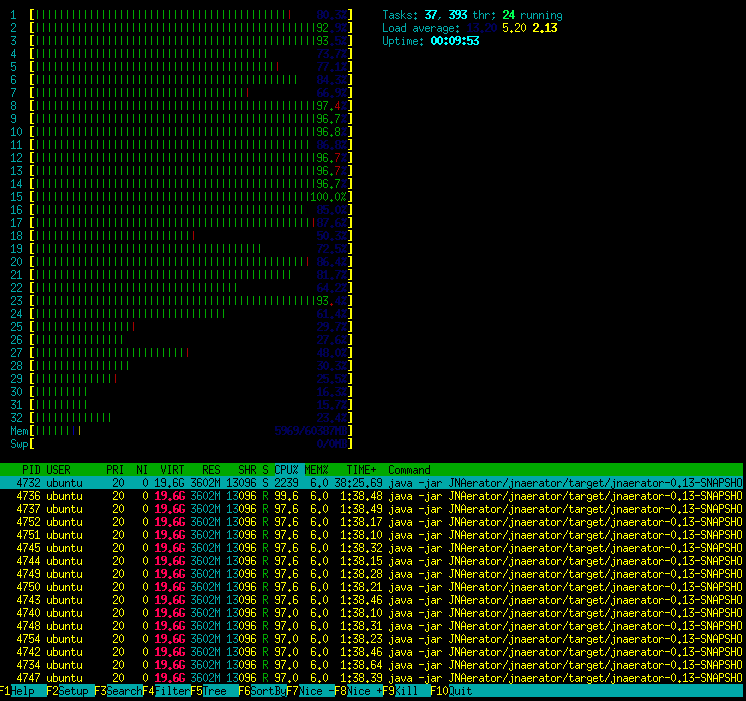
\includegraphics[width=\linewidth]{parallel_parsing.png}
\end{frame}

\end{document}
